\chapter{Governo Aberto}

De acordo com Daniela Siva~\cite{silva}, A publicidade dos atos de governo é um princípio democrático, que no Brasil aparece expressa no artigo 5º da Constituição: “todos são iguais perante a lei, sem distinção de qualquer natureza, garantindo-se aos brasileiros e aos estrangeiros residentes no País a inviolabilidade do direito à vida, à liberdade, à igualdade, à segurança e à propriedade”. No inciso XXXIII deste artigo, determina-se que “todos têm direito a receber dos órgãos público informações de seu interesse particular, ou de interesse coletivo ou geral, que serão prestadas no prazo da lei, sob pena de responsabilidade, ressalvadas aquelas cujo sigilo seja imprescindível à segurança da sociedade e do Estado”. No artigo 37 da Constituição, fica explícito que “a administração pública direta e indireta de qualquer dos Poderes da União, dos estados, do distrito federal e dos municípios obedecerá aos princípios de legalidade, impessoalidade, moralidade, publicidade e eficiência”. 

Atualmente, com avanço tecnológico que estamos sofrendo, surgem diversas ferramentas que aumentam a capacidade da sociedade em assumir seus direitos e obrigações cívicas. A inclusão digital, a informatização dos procedimentos governamentais e a integração entre diversos repositórios de dados públicos gera crescentes demandas da população por mais transparência e participação através de meios tecnológicos.

Mesmo com o crescente interesse da sociedade atual nos dados públicos e com o amparo da constituição, até então no Brasil ainda não existiam leis específicas que determinassem prazos e formas para que o poder público atenda a pedidos de informação pública por parte da comunidade.

Em 2011, foi sancionada a lei Nº 12.527, mais conhecida como lei de acesso a informação\cite{lai}. Foi a primeira lei criada que trata de acesso as informações públicas. Antes de ser aprovada, ela passou por algumas reformulações sugeridas pela comunidade Hacker, afim de garantir o acesso a dados abertos. A lei engloba todos os oito princípios de dados abertos. 

Ainda de acordo com Daniela Silva\cite{silva}, os “Governos e departamentos interessados em fazer a abertura de seus dados, portanto, podem seguir como princípio as determinações do projeto de Lei de Acesso à Informação Pública, que está de acordo com as possibilidades de gerar cruzamentos, visualizações e serviços garantidos pelas novas tecnologias em rede.”

\section{INDA}
\label{sec-proc-sl}

A lei de acesso a informação \cite{lai}  foi o pontapé inicial para várias iniciativas na área de dados abertos governamentais (OGD\footnote{OGD - Disponível em: \url{http://opengovernmentdata.org/}.} – open government data). Hoje, o governo vem promovendo diversas ações tanto na esfera administrativa quanto na legislativa, dando apoio a abertura de dados. 

Em 13 de abril de 2012, foi publicado no Diário Oficial da União (DOU), a instrução normativa de Nº 4 que institui o Plano de Ação Nacional sobre Governo Aberto, o qual estabelece o compromisso do governo de implantar a Infraestrutura Nacional de Dados Abertos - INDA.

Como disposto no site de dados abertos do governo federal, a INDA é um conjunto de padrões, tecnologias, procedimentos e mecanismos de controle necessários para atender às condições de disseminação e compartilhamento de dados e informações públicas no modelo de Dados Abertos, em conformidade com o disposto na e-PING\footnote{e-PING - Padrões de Interoperabilidade de Governo Eletrônico. Disponível em:\url{ http://eping.governoeletronico.gov.br/}}. A INDA é a política do governo brasileiro para dados abertos.

Todas essas diretrizes da INDA são melhores descritas no seu plano de ação \cite{planoinda}. Esse plano apresenta três finalidades principais:

\begin{itemize}

\item {Auxiliar as organizações integrantes da INDA a cumprir a Lei de Acesso à Informação, no que se refere à transparência ativa pela publicação de dados governamentais abertos; }

\item {Nortear os órgãos e entidades integrantes da INDA, quanto à visão, estratégia e política de abertura de dados na administração pública federal, para os anos de 2013 e 2014; }

\item {Servir como base para criação de planos de publicação de dados abertos na INDA, conforme disposto no Art. 6º, VII, alínea c da Instrução Normativa 04 de 12 de abril de 2012.}

\end{itemize}

\graphicspath{{figuras/}}
\begin{figure}[H]
\centering
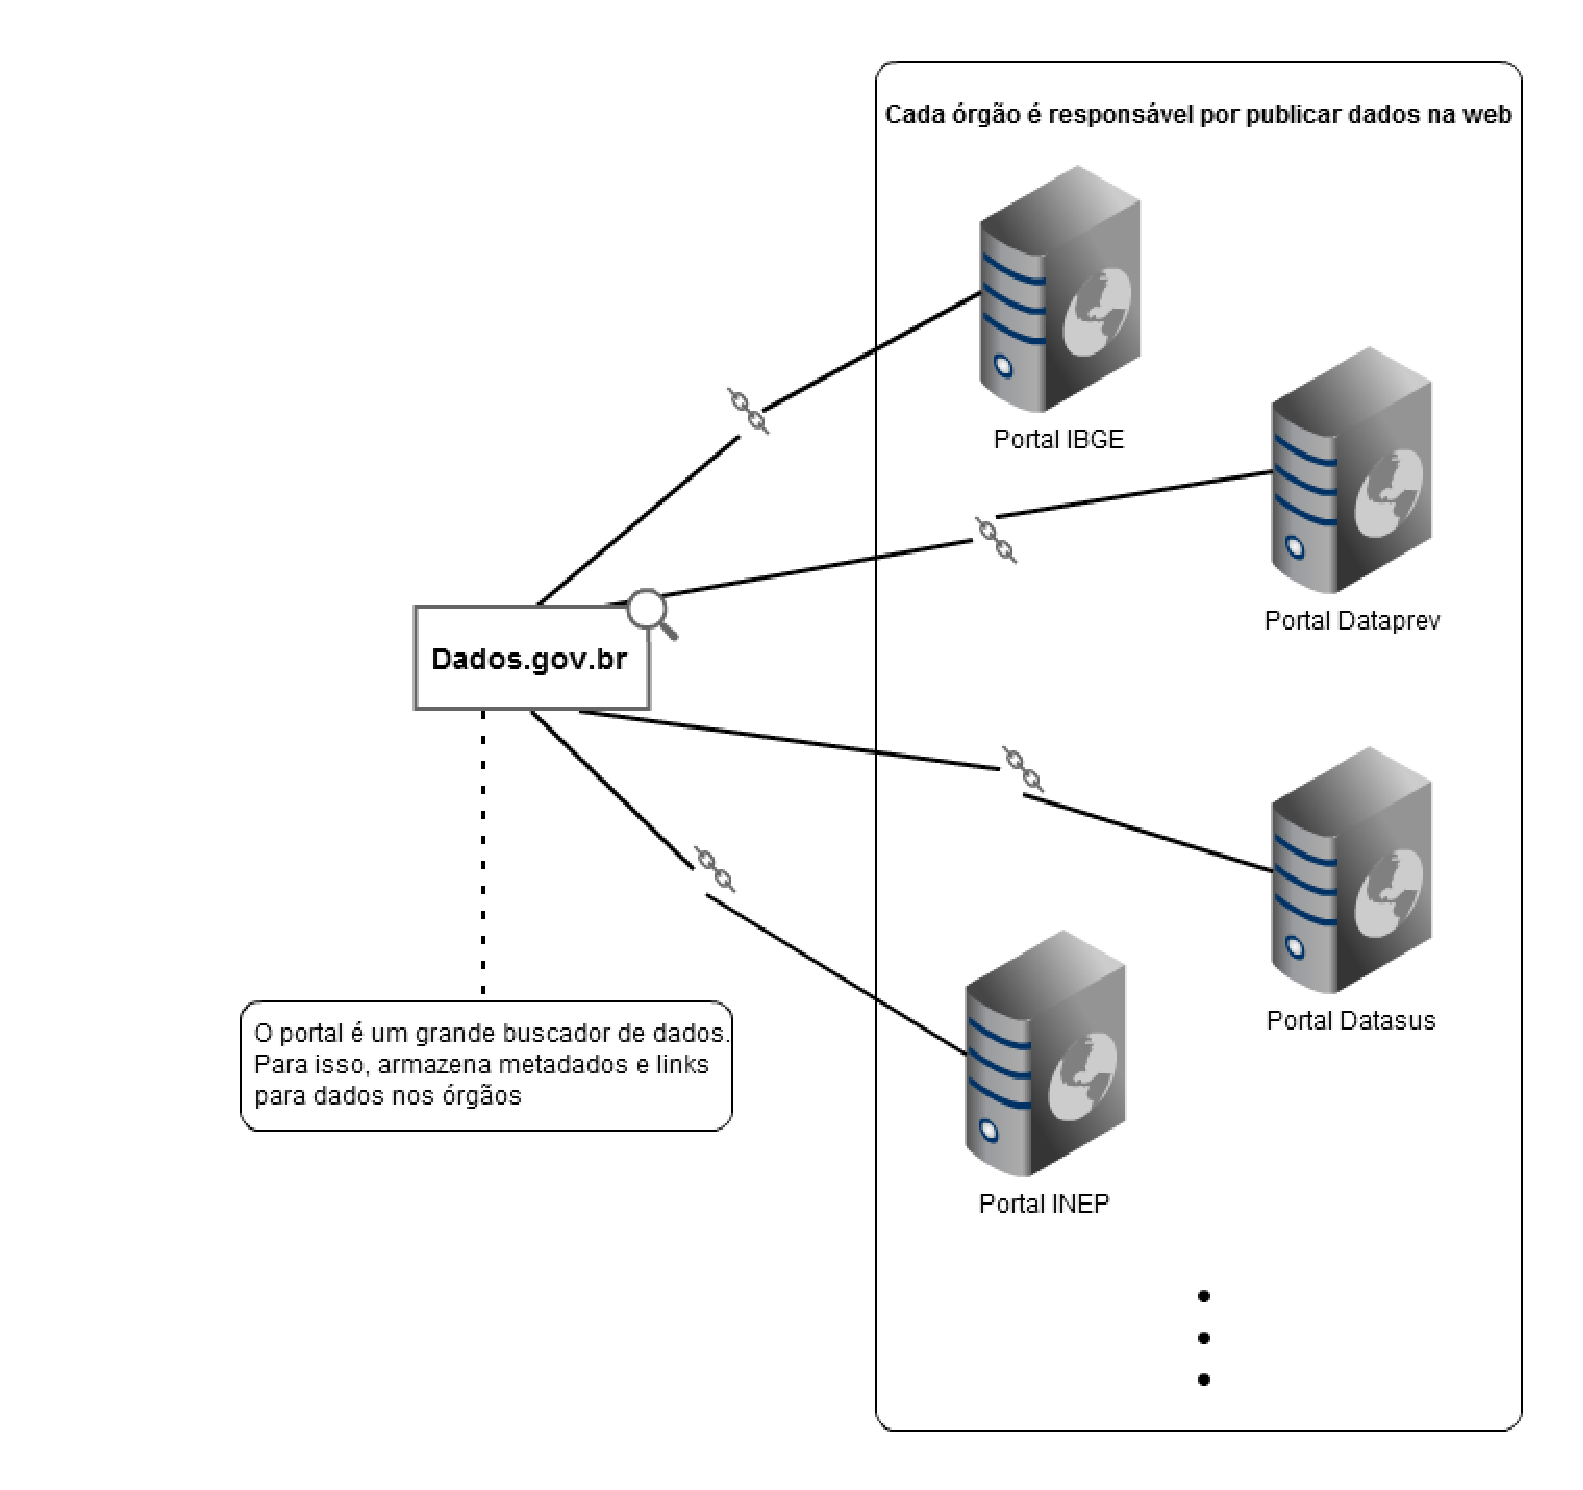
\includegraphics[width=0.8\textwidth]{plano_acao}
\caption[Diagrama de implantação da INDA.]{Diagrama de implantação da INDA. Extraído de \cite{planoinda}}
\label{plano_acao}
\end{figure}

Como podemos ver na figura \ref{plano_acao}, a INDA é responsável por manter o portal brasileiro de dados abertos. Esse portal é um catálogo central que mantém um conjunto de metadados sobre as informações disponibilizadas pelas organizações da INDA. Informações como nome do dado, URL (ou endereço web) do dado, autor do dado, responsável pela manutenção do dado, formato do dado (odt, csv, json, xml, etc) são catalogadas para garantir que o usuário encontre o que está procurando. 

Desse modo, o portal funcionará como um grande buscador de dados. Cada organização participante da INDA será responsável por publicar seus dados na web através de portal próprio, cadastrar seus metadados no portal(endereço, nome, data da coleta, assunto, etc) e posteriormente garantir a disponibilidade desses dados em seu ambiente próprio.

Para que essas organizações possam participar da INDA, elas deverão seguir uma serie de recomendações para que os dados disponibilizados sejam mais úteis, reutilizáveis e fáceis de encontrar. Um importante documento que contém inúmeras boas práticas para esse processo de publicação é a Cartilha Técnica 	para publicação de Dados Abertos \cite{cartilha}, disponível no portal.

\graphicspath{{figuras/}}
\begin{figure}[H]
\centering
\includegraphics[width=0.9\textwidth]{portal}
\caption[Portal de dados abertos.]{Portal de dados abertos. Extraído de \cite{dadosabertos} }
\label{portal}
\end{figure}

\section{OGP}
\label{sec-padroes-sl} 

A parceria para Governo Aberto ou OGP\footnote{OGP - Disponível em: \url{http://www.opengovpartnership.org/}} (do inglês open Government Partnership), lançada em 2011, é uma iniciativa internacional que pretende difundir e incentivar globalmente práticas governamentais relacionadas a transparência dos governos, ao acesso à informação pública e à participação social \cite{mapaogp}.

Inicialmente ela foi composta por oito países: África do sul, Brasil, Estados unidos, Filipinas, Indonésia, México, Noruega e Reino Unido. Esses países são considerados os fundadores da OGP. Eles oficializaram essa parceria quando assinaram a Declaração de Governo Aberto e apresentaram seus planos de ação. Atualmente, a OGP conta com 63 países.

\graphicspath{{figuras/}}
\begin{figure}[H]
\centering
\includegraphics[width=1.0\textwidth]{mapa_OGP}
\caption[Países participantes da OGP.]{Países participantes da OGP. Extraído de \cite{mapaogp} }
\label{portal}
\end{figure}

Como um dos co-fundadores da OGP, o Brasil está fortemente empenhado em reforçar a transparência das ações do governo, prevenção e combate à corrupção, a promoção dos ideais democráticos com a participação dos cidadãos na tomada de decisões e melhoria dos serviços públicos. Ao longo dos últimos 10 anos, o país desenvolveu várias iniciativas para melhorar o seu quadro legal, a participação do cidadão e fomentar o uso da tecnologia para uma maior abertura.

Todas as medidas a serem executadas pelo Brasil, ficam registradas em seu plano de ação. No primeiro plano, o Brasil se comprometeu com 32 compromissos. O país conseguiu implementar total ou parcialmente cerca de 90% desses compromissos gerando alguns benefícios como: a criação do Portal de Dados Abertos, da organização da conferência nacional sobre transparência (CONSOCIAL) – que envolveu mais de 100.000 cidadãos - e por fim a implementação da lei de acesso a informação brasileiro.

Responsável com congregar nações e organizações da sociedade civil líderes em transparência e governo aberto, a OGPé um veículo para se avançar mundialmente no fortalecimento das democracias e dos direitos humanos, na luta contra a corrupção e no fomento de inovações e tecnologias para transformar a governança do século XXI mais transparente.



